\documentclass{article}

% if you need to pass options to natbib, use, e.g.:
%     \PassOptionsToPackage{numbers, compress}{natbib}
% before loading neurips_2021

% ready for submission
% \usepackage{neurips_2021}

% to compile a preprint version, e.g., for submission to arXiv, add add the
% [preprint] option:
%     \usepackage[preprint]{neurips_2021}

% to compile a camera-ready version, add the [final] option, e.g.:
\usepackage[final]{neurips_2021}

% to avoid loading the natbib package, add option nonatbib:
%    \usepackage[nonatbib]{neurips_2021}

\usepackage[utf8]{inputenc} % allow utf-8 input
\usepackage[T1]{fontenc}    % use 8-bit T1 fonts
\usepackage{hyperref}       % hyperlinks
\usepackage{url}            % simple URL typesetting
\usepackage{booktabs}       % professional-quality tables
\usepackage{amsfonts}       % blackboard math symbols
\usepackage{nicefrac}       % compact symbols for 1/2, etc.
\usepackage{microtype}      % microtypography
\usepackage{xcolor}         % colors
\usepackage{graphicx}
\usepackage{float}

\title{ELEC 400m Final Project}


\author{%
  Matthew C. Sam \\
  Department of Electrical and Computer Engineering\\
  University of British Columbia\\
  Vancouver, BC V6T 1Z4\\
  \texttt{mattsam@student.ubc.ca} \\
}

\begin{document}

\maketitle
\begin{abstract}
    In my project I perform classification of a zoo animal dataset from Kaggle using 3 different methods. I attempt to tune the hyperparameters of each method leveraging using cross-validation. Performance of the models that had the highest accuracy on the training data is evaluated on new testing data. The results of each model are compared, and over/under fitting of the models is discussed.
\end{abstract}

\section{Introduction}
    The base "Zoo Animal Classification" dataset is a set of 102 different Animals split into 7 classes with 16 features assigned to each animal. The animals are separated by features (table 1) and their classes are based roughly on their taxonomy class (table 2).
    \begin{table}[H]
      \caption{Features}
      \label{feature-table}
      \centering
      \begin{tabular}{lll}
        \cmidrule(r){1-2}
        Feature Number & Feature Name   & Value type          \\
        \midrule
        1    & has hair                 & 1/0               \\
        2    & has feathers             & 1/0               \\
        3    & lays eggs                & 1/0               \\
        4    & produces milk            & 1/0               \\
        5    & can fly                  & 1/0               \\
        6    & aquatic or semi-aquatic  & 1/0               \\
        7    & carnivorous              & 1/0               \\
        8    & has teeth                & 1/0=              \\
        9    & has a backbone           & 1/0               \\
        10   & Respires with Lungs      & 1/0               \\
        11   & venomous or poisonous    & 1/0               \\
        12   & Fins                     & 1/0               \\
        13   & Legs                     & number of legs    \\
        14   & Tail                     & 1/0               \\
        15   & Domesticated             & 1/0               \\
        16   & cat sized                & 1/0               \\
        \bottomrule
      \end{tabular}
    \end{table}
    The 7 classes are: 
    \begin{table}[H]
      \caption{Classes}
      \label{class-table}
      \centering
      \begin{tabular}{ll}
        \cmidrule(r){1-2}
        Class Number     & Class Name      \\
        \midrule
        0   & Mammals   \\
        1   & Birds   \\
        2   & Reptiles   \\
        3   & Fish   \\
        4   & Amphibians   \\
        5   & Insects  \\
        6   & Non-insect Invertebrates  \\
        \bottomrule
      \end{tabular}
    \end{table}

    The distribution of classes in the base dataset was as follows
    \begin{figure}[H]
      \centering
      \fbox{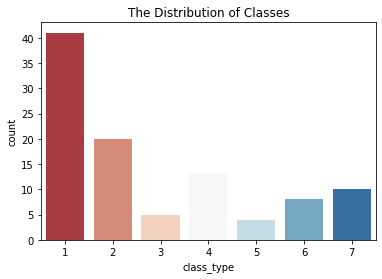
\includegraphics[width=5cm]{Class_distribution.png}}%
      \caption{Distribution of Classes In Training Data}
    \end{figure}

\section{Methods/Applications}
\subsection{Code Structure}
\subsubsection{Data Collection and Preprocessing}
\paragraph{}
    This dataset was found on Kaggle first by setting the filter to "classification" then looking for datasets related to animals since I felt that for myself it would be interesting to do classification of animals based on features. 
    

\paragraph{}
    I used Kaggle's API to download the dataset into Google Colab in order to start working on it. It came as a zipped CSV file which I unzipped and loaded into a dataframe. The dataframe was then split into X and Y (features and classes) and split further into a training and test split of 80:20, when I say "training data" I am referring to the model that is trained on the training split and the resulting predictions on the "test" split. When I refer to "test" data I mean the extra dataset that. Before starting I looked at the contents of the dataset and put them on a bar graph in order to see if any of the classes had less samples. I saw that the 3rd class (reptiles) only had 3 samples. Seeing this, I set up a weight dictionary with the distribution of classes for experimenting on later.
    
\subsection{Model Overview}
\paragraph{}
    The three classification methods that I chose to use were Random Forest, Logistic Regression, and K Nearest Neighbors. I chose these 3 in order to have a mix of supervised and unsupervised methods.
    
\subsubsection{Random Forest}
\paragraph{}
    In total, 6 models were trained. For each model, the accuracy of the 8:2 split was measured as well as the mean cross validation score. Different number of estimators, criterion, and the addition of class weights were tested to try to find the optimal setting for each parameter.
    
    \begin{figure}[H]
      \centering
      \fbox{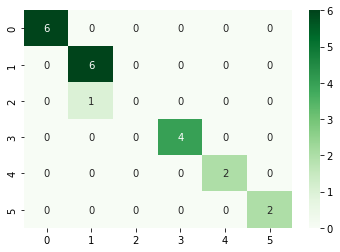
\includegraphics[width=5cm]{RF_cn_train.png}}%
      \caption{Confusion Matrix From Best RF Model On Training Data}
    \end{figure}
\subsubsection{Logistic Regression}
\paragraph{}
    In total, 12 models were trained. As with random forest, the accuracy of the 8:2 split was measured as well as the mean cross validation score. The first model was using the same settings that were used in the first homework assignment. I experimented with different penalties, adding class weights, and different solvers.
    
    \begin{figure}[H]
      \centering
      \fbox{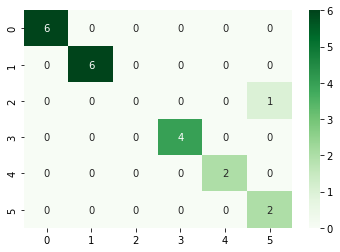
\includegraphics[width=5cm]{LR_cf_train.png}}%
      \caption{Confusion Matrix From Best RF Model On Training Data}
    \end{figure}
\subsubsection{K Nearest Neighbors}
\paragraph{}
    For KNN, the only parameter that was changed in each model was the number of neighbors. 15 models were trained with n in the range (1,15). Although a n of 1 should lead to obvious over fitting to training data, I was curious as to how it would perform on the separate testing dataset.

    \begin{figure}[H]
      \centering
      \fbox{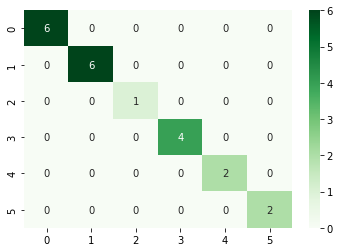
\includegraphics[width=5cm]{Knn_cf_train.png}}%
      \caption{Confusion Matrix From Best KNN Model On Training Data}
    \end{figure}
\section{experiment/results}
\subsection{Random Forest Model Performance On Test Data}
\paragraph{} 
    For random forest, the first model was essentially just a decision tree classifier and as expected it did not outperform the multiple n valued RF models. However, something that I did not predict was that models 2, 3, and 5 would all have the same performance (based on the accuracy from cross validation). This showed that the jump form 10 to 100 estimators was negligible in terms of accuracy. After seeing that this was the difference in models 2 and 3 I was not as surprised. The difference in model 5 was that model 5 had 10 estimators but was also given class weights. So even though they showed the same performance on the training dataset if they have differences on the larger testing dataset, I would think that model 5 would exhibit some over fitting but on the test data, model 3 and 5 had similar performance (both with an accuracy score of 0.9026548672566371), but model 2 actually ended up performing worse (accuracy score of 0.8761061946902655).

    \begin{figure}[H]
      \centering
      \fbox{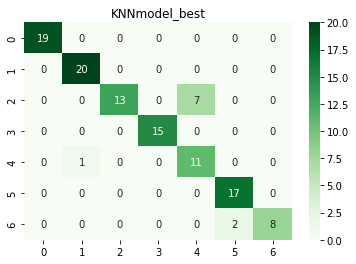
\includegraphics[width=5cm]{Knn_cf.png}}%
      \caption{Confusion Matrix From Best KNN Model on Test Data}
    \end{figure}

\subsection{Logistic Regression Model Performance On Test Data}
\paragraph{}
    For logistic regression not having any penalty ended up being the most accurate penalty on the training data, and accuracy appeared to be solver agnostic. As expected, when model weights were given the model was able to perfectly predict the test data, and had slightly better performance in accuracy using cross validation. With the weights inverted, the performance was the same as if there were no weights given at all. The model that I deemed the best was that with no penalty using the default solver and no weights.
    
    \begin{figure}[H]
      \centering
      \fbox{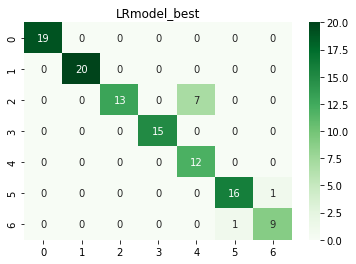
\includegraphics[width=5cm]{LR_cf.png}}%
      \caption{Confusion Matrix From Best Logistic Regression Model on Test Data}
    \end{figure}
\subsection{K Nearest neighbors Model Performance On Test Data}
\paragraph{}
    The KNN models were the easiest to test. Since the square root of the number of samples is a good ballpark estimate for optimal k I created an array of values around the range of 10. The cross validation accuracy pointed towards a k of 1 being optimal which seemed wrong to me so I went on to compare the performance of k = 1,3,5 just in case it was badly over fit. To my surprise, even on the seperate test dataset k = 1 performed the best.
    \begin{figure}[H]
      \centering
      \fbox{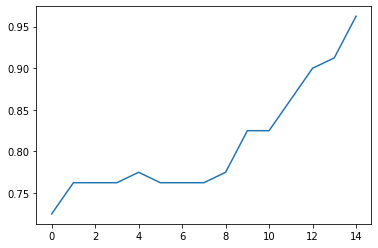
\includegraphics[width=5cm]{knn_n.png}}%
      \caption{Accuracy vs k value}
    \end{figure}
    \begin{figure}[H]
      \centering
      \fbox{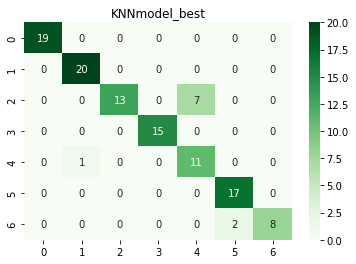
\includegraphics[width=5cm]{Knn_cf.png}}%
      \caption{Confusion Matrix From Best KNN Forest Model on Test Data}
    \end{figure}

\section{Discussion}
\subsection{Model Comparison}
\paragraph{}
    Looking at the resulting metrics of the three best models from each of the methods logistic regression. As seen in table 3, Logistic regression performed the best in all metrics in my experiments.
        \begin{table}[H]
      \caption{Features}
      \label{feature-table}
      \centering
      \begin{tabular}{llll}
        \cmidrule(r){1-2}
       & Random Forest & Logistic Regression & K Nearest Neighbors \\
        \midrule
        accuracy score      & 0.90265 & 0.92035 & 0.91150 \\
        macro recall        & 0.89285 & 0.92731 & 0.90952 \\
        micro recall        & 0.90265 & 0.92035 & 0.91150 \\
        weighted recall     & 0.90265 & 0.92035 & 0.91150 \\
        macro precision     & 0.92015 & 0.92467 & 0.92260 \\
        micro precision     & 0.90265 & 0.92035 & 0.91150 \\
        weighted precision  & 0.93221 & 0.94317 & 0.93443 \\
        macro f1            & 0.88668 & 0.91474 & 0.90430 \\
        macro f1            & 0.90265 & 0.92035 & 0.91150 \\
        weighted f1         & 0.90051 & 0.92077 & 0.91163 \\
        \bottomrule
      \end{tabular}
    \end{table}
\paragraph{}
    In the confusion matrices it can be seen that in all models there are 7 false positives where reptile is predicted but the sample is actually an amphibian. After seeing the class distribution in the training data it isn't that surprising since reptiles and amphibians have several traits that are common in both classes while both classes having less samples than the others. One possible solution to this issue would be to augment the dataset to bring all of the samples to a more even distribution.

\section{Conclusion}
\paragraph{}
    Although logistic regression did outperform the other two methods there are some shortcomings in my experiments I wish to address. Aside from the aforementioned small sample size of reptiles and amphibians, I left the cv as 4 in all experiments to make sure all of the samples would have at least one of each class. In hindsight I think doing tests where cv is more than 4 would have been beneficial. 
\label{headings}

\section*{References}

{
\small

UCI MACHINE LEARNING. (2016). Zoo Animal Classification, [Version of the dataset]. Retrieved December 2022 from https://www.kaggle.com/datasets/uciml/zoo-animal-classification.

RODRIGO HJORT. (2018). Zoo Animals Extended Dataset, [Version of the dataset]. Retrieved December 2022 from https://www.kaggle.com/datasets/agajorte/zoo-animals-extended-dataset.


}

\end{document}